\section{Implementação}
\label{sec:implementation}
Para comparar os sistemas que utilizam apenas um banco de dados, persistência monoglota, com os sistemas que utilizam mais de um banco de dados, persistência poliglota, implementamos e testamos o desempenho desses.

Escolhemos fazer uma aplicação semelhante ao Twitter. Nessa aplicação o usuário poderá se cadastrar, escrever \textit{tweets}, seguir outros usuários e listar os \textit{tweets} dos usuários que ele segue. Para descrever essas funcionalidades segue os casos de uso abaixo:

\textbf{Caso de Uso 1 - Cadastro do usuário}

Sumário: Usuário usa o sistema para se cadastrar

Ator primário: Usuário

Ator secundário: Sistema

Precondições: O usuário deverá ter uma email

Fluxo Principal

\begin{enumerate}
\item O usuário acessa o sistema
\item O sistema exibe a tela de entrada
\item O usuário clica em \textit{Sign up}
\item O sistema retorna a tela com o formulário de cadastro de usuário
\item O usuário preenche os campos de nome, email, senha e confirmação de senha
\item O sistema cria o usuário e redireciona para tela de \textit{My Tweets}
\end{enumerate}

Fluxo de Exceção (5): Email inválido
\begin{enumerate}
\item Se o usuário não digitou um email válido, o sistema reporta o campo incorreto e retorna ao passo 5.
\end{enumerate}

Fluxo de Exceção (5): Campos obrigatórios não preenchidos
\begin{enumerate}
\item Se o usuário não preencher todos os campos, o sistema informa que os campos são obrigatórios e o usuário retorna ao passo 5.
\end{enumerate}

Fluxo de Exceção (5): Senha e confirmação de senha não conferem
\begin{enumerate}
\item Se o usuário não preencher as senhas corretamente, o sistema retorna ao passo 5, informando que as senhas não conferem.
\end{enumerate}


\textbf{Caso de Uso 2 - Cadastro de \textit{tweet}}

Sumário: Usuário usa o sistema para cadastrar um \textit{tweet}

Ator primário: Usuário

Ator secundário: Sistema

Precondições: O usuário deverá ser cadastrado e deve estar logado no sistema

Fluxo Principal
\begin{enumerate}
\item O usuário acessa o sistema e faz o \textit{login}
\item O sistema abre a listagem dos \textit{tweets} do usuário
\item O usuário clica no botão \textit{New Tweet}
\item O sistema retorna com o formulário para cadastrar \textit{tweet}
\item O usuário escreve o \textit{tweet} no campo indicado
\item O sistema cria um novo \textit{tweet}, registrando que o usuário é o autor do \textit{tweet}, data e hora que foi criado
\end{enumerate}

\textbf{Caso de Uso 3 - Usuário segue outro usuário}

Sumário: Usuário segue outro usuário

Ator primário: Usuário

Ator secundário: Sistema

Precondições: O usuário deverá ser cadastrado e deve estar logado no sistema

Fluxo Principal
\begin{enumerate}
\item O usuário acessa o sistema e faz o \textit{login}
\item O sistema abre a listagem dos \textit{tweets} do usuário
\item O usuário clica no menu \textit{Users}
\item O sistema retorna a listagem paginada com todos os usuários cadastrados
\item O usuário escolhe algum usuário que deseja seguir e clica no botão \textit{Follow}
\item O sistema armazena essa informação
\end{enumerate}

\textbf{Caso de Uso 4 - Usuário para de seguir algum usuário}

Sumário: Usuário para de seguir algum usuário

Ator primário: Usuário

Ator secundário: Sistema

Precondições: O usuário deverá ser cadastrado e deve estar logado no sistema. Além disso, o usuário logado deve estar seguindo o usuário que ele deseja parar de seguir

Fluxo Principal
\begin{enumerate}
\item O usuário acessa o sistema e faz o \textit{login}
\item O sistema abre a listagem dos \textit{tweets} do usuário
\item O usuário clica no menu \textit{Users}
\item O sistema retorna a listagem paginada com todos os usuários cadastrados
\item O usuário encontra o usuário que deseja parar seguir e clica no botão \textit{Unfollow}
\item O sistema armazena essa informação
\end{enumerate}

\textbf{Caso de Uso 5 - Usuário visualiza a \textit{feed}}

Sumário: Usuário visualiza os \textit{tweets} dos usuários que ele segue

Ator primário: Usuário

Ator secundário: Sistema

Precondições: O usuário deverá ser cadastrado e deve estar logado no sistema. Além disso, o usuário logado deve estar seguindo algum usuário

Fluxo Principal
\begin{enumerate}
\item O usuário acessa o sistema e faz o \textit{login}
\item O sistema abre a listagem dos \textit{tweets} do usuário
\item O usuário clica no menu \textit{Feed}
\item O sistema retorna a listagem paginada com todos os \textit{tweets} dos usuários que o ator primário segue.
\end{enumerate}

Ambos os sistemas foram desenvolvidos na linguagem \textit{ruby} com o \textit{framework rails}. Esse \textit{framework} é próprio para Web e utiliza a arquitetura de \textit{software} \ac{MVC}. Além disso, é uma ferramenta de desenvolvimento ágil, que facilita o desenvolvimento Web.
Foram utilizado outras \textit{gems}, a lista utilizada em cada aplicação criada se encontra no arquivo chamado Gemfile.lock. Podemos destacar a gem Devise \footnote{\url{https://github.com/plataformatec/devise}} e a gem MongoId \footnote{\url{http://mongoid.org/}} como principais. A Devise faz o controle de sessão do usuário e a Mongoid deixa transparente para o desenvolvedor a comunicação com o banco de dados MongoDB. Também utilizamos a gem bootstrap-sass para melhorar usabilidade da aplicação.

A diferença dos sistemas se descreve nas seções seguintes.

\section{Implementação Monoglota}
\label{sec:monoglot}

Essa implementação utiliza apenas o banco de dados MongoDB que é orientado a documento.

Na camada de modelos temos apenas duas classes, \verb|Tweet| e \verb|User|. A classe \verb|Tweet| representa o \textit{tweet} e a classe \verb|User| representa o usuário. Ambos são armazenados como coleção no MongoDB. Cada objeto de uma dessas classes é um documento. Na \autoref{fig:diagrama_models} podemos visualizar o relacionamento entre as classes.
\begin{figure}[H]
    \centering
    \caption{Camada de controle}
    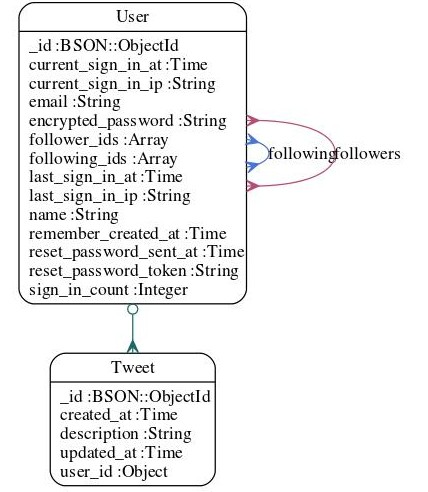
\includegraphics[width=0.5\textwidth]{./04-figuras/models_complete.jpg}
    \fonte{\cite{NoSQL}}
    \label{fig:diagrama_models}
\end{figure}
A classe \verb|Tweet| armazena identificador do próprio \textit{tweet}, data de criação, data da ultima atualização desse objeto, descrição do \textit{tweet} e o identificador do usuário que criou o \textit{tweet}. Não escolhemos usar agregação nessa relação, pois umas das principais perspectivas é visualizar os \verb|Tweets| de diferentes usuários. Nessa classe temos duas validações uma de presença do campo descrição e outra que limita o tamanho desse campo em cento e quarenta caracteres.

A classe \verb|User| armazena o identificador do usuário, email, nome, uma série de campos usados para autenticação, data de criação do objeto, data da última modificação do objeto, lista de usuários seguidos e a lista de usuários seguidores. A classe \verb|User| tem três relacionamentos, um com \verb|Tweet| que já foi citado e dois autorrelacionamentos para armazenar a lista de usuários que seguem e que são seguidos. Esse autorrelacionamento no banco de dados orientado a documento funciona de uma maneira diferente do banco de dados relacional.
Enquanto no modelo relacional é necessário criar uma nova tabela, no modelo não-relacional armazenamos apenas as listas com os identificadores dos usuários, pois é permitido valores multivalorados. Logo, basta armazenar os identificadores da relação em uma lista embutida no documento do usuário. Então temos uma lista que armazena os identificadores dos usuários que são seguidos, chamada de \verb|following| e outra lista com os identificadores dos usuários que são seguidores, chamada de \verb|followers|.
Essa classe tem três validações de presença: uma para o campo nome, outra para o campo email e a terceira para o campo de senha.

Na camada de controle temos uma hierarquia conforme mostra a \autoref{fig:diagrama_controllers}. \verb|ApplicationController| é a classe de controle que herda da classe do \textit{framework}. Em seguida, temos o \verb|HomeController| e \verb|Logged::BaseController| que herda  da classe \verb|ApplicationController|. \verb|HomeController| é a classe responsável por implementar o controle das páginas de \verb|about| e \verb|index|. Já o \verb|Logged::BaseController| é a classe responsável por carregar o layout do usuário logado e verificar a autenticidade do usuário.
Abaixo do \verb|Logged:BaseController| foram criadas mais duas classes: \verb|TweetsController| e \verb|UsersController| que implementam os controles de \textit{tweets} e usuários respectivamente.
\begin{figure}[H]
    \centering
    \caption{Camada de controle}
    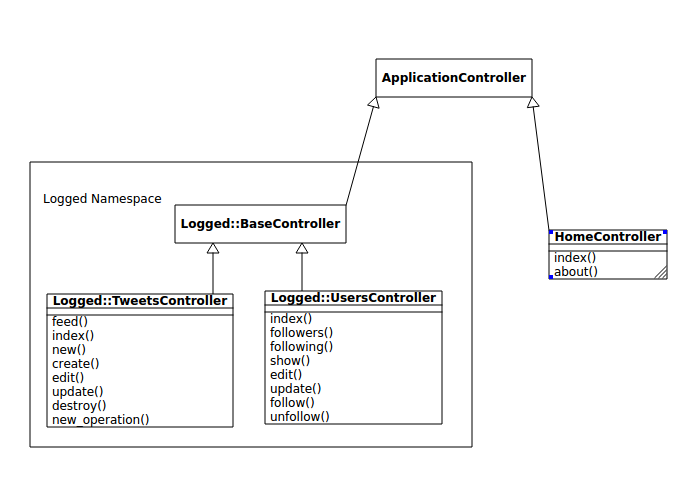
\includegraphics[width=0.8\textwidth]{./04-figuras/controllers_complete.png}
    \fonte{\cite{NoSQL}}
    \label{fig:diagrama_controllers}
\end{figure}

Todas as listas são paginadas de trinta em trinta e antes de todas ações é executado uma consulta, no banco, que carrega para variável \verb|current_user| o usuário logado. Essa busca é feita pela \textit{gem} Devise e é transparente para o desenvolvedor.

O controle de usuário implementa as ações \verb|index|, \verb|followers|, \verb|following|, \verb|show|, \verb|edit|, \verb|update|, \verb|follow| e \verb|unfollow|.

A ação \verb|index| lista todos os usuários com exceção do usuário logado. Na página renderizada o usuário logado poderá seguir os usuários que ele ainda não segue, ou poderá parar de seguir os usuários que ele segue. É realizado apenas uma consulta para ler os usuários do sistema.

A ação \verb|followers| lista todos os usuários que seguem o usuário logado. Na página renderizada, o usuário logado poderá seguir os usuários que ele ainda não segue, ou poderá parar de seguir os usuários que ele já segue. É realizado apenas uma consulta no banco de dados que busca todos os usuários que o usuário logado segue.

A ação \verb|followings| lista todos os usuários que o usuário logado segue. Na página renderizada, o usuário logado poderá parar de seguir os usuários que ele segue. Da mesma maneira que a ação \verb|followers|, é realizado apenas uma consulta, porém busca os usuários que seguem o usuário logado.

A ação \verb|show| recebe um identificador como parâmetro e localiza o usuário que possui esse identificador. A página renderizada mostra o nome e email do usuário localizado e os tweets que ele fez. Nessa página são realizadas duas consultas, uma que busca o usuário e outra que busca os \textit{tweets} desse usuário.

A ação \verb|edit| renderiza o formulário de edição para que o usuário logado possa mudar algum campo, como nome, email ou senha. Nessa ação nenhuma consulta adicional é feita.

A ação \verb|update| recebe os parâmetros das alterações que o usuário fez no próprio perfil e registra isso no banco de dados. É realizado uma escrita no banco de dados para atualizar esses dados passados por parâmetro.

A ação \verb|follow| recebe como parâmetro o usuário que será seguido pelo usuário logado e registra esse relacionamento. Para isso é necessário uma consulta para ler qual usuário será seguido e duas escritas: uma para atualizar o usuário que está sendo seguido com o identificador do usuário seguidor e outra para atualizar o usuário seguidor com o identificador do usuário seguido.

A ação \verb|unfollow| recebe como parâmetro o usuário que deixará de ser seguido pelo usuário logado e apaga o registro desse relacionamento. Para isso é necessário uma consulta para ler o usuário que deixará de ser seguido e duas escritas no banco de dados: uma para atualizar a lista de seguidores do usuário que deixou de ser seguido outra para atualizar a lista de seguindo do usuário seguidor que deixou de seguir.

O controle de tweets implementa as ações feed, index, new, edit, update e destroy.

A ação feed é responsável por fazer a busca no banco de dados dos tweets de todos os usuários que o usuário logado segue, ordenado pelos tweets mais recentes.

A ação de index lista todos os tweets do usuário logado, para isso foi necessário fazer apenas uma consulta no banco de dados que busca esses tweets.

A ação new renderiza o formulário de cadastro de tweet, não é feito nehuma consulta adicional.

A ação create recebe como parâmetro o campo de descrição do tweet, relaciona esse tweet com o usuário logado e faz a escrita no banco desse tweet caso seja válido.

A ação update recebe como parâmetro o campo de descrição e o id do tweet que será alterado, faz a leitura no banco de dados desse tweet com o id passado. Em seguida, altera o valor da descrição e faz a escrita no banco de dados.

A ação destroy recebe como parâmetro o id do tweet que será excluído, em seguida faz a leitura desse tweet para verificar se o usuário logado é o dono do tweet e caso seja confirmado faz exclusão desse tweet no banco de dados.



\section{Implementação Poliglota}
\label{sec:polyglot}

Na aplicação monoglota a única maneira de consultar os tweets da feed é buscar todos os tweets, cujo o autor esteja na lista de followers do usuário logado. Para isso era necessário varrer tweet por tweet e verificar se o autor está na lista. Pensando nessa abordagem utilizamos a persistência poliglota para melhorar o tempo de leitura da feed.
Então utilizamos um segundo banco de dados do gênero chave-valor, chamado \ac{Redis}, que irá armazenar os cem tweets mais recentes, cujo o autor está na lista de followers do usuário logado.
O \ac{Redis} irá armazenar esses cem tweets em uma chave com o id do usuário concatenada com a string \"\_feed\", ou seja, o usuário que tem o id igual a um, a chave será \"1\_feed\". Todo usuário terá uma chave que armazenará os tweets da feed. Quando ele for acessar a página de feed, ao invés do sistema fazer a consulta no MongoDB e varrer tweet por tweet, ele irá apenas consultar o \ac{Redis} com a chave e será retornado o valor com todos os tweets da feed.


Para persistir esses dados no \ac{Redis} precisamos de alterar o sistema. Inicialmente foi necessário instalar outra gem, chamada redis \footnote{\url{https://github.com/antirez/redis}}, que faz a comunicação com o banco de dados chave-valor. Em seguida, implementamos três métodos na classe \verb|User|: feed\_key, remake\_feed e update\_tweet\_hash.

O método feed\_key foi criado apenas para retornar a chave que será usada para armazenar no \ac{Redis}.

O método remake\_feed foi criado para refazer o valor da feed de algum usuário quando necessário. Após fazer a implementação poliglota, utilizamos esse método para popular o \ac{Redis}.

O método update\_tweet\_hash foi implementado para adicionar mais um tweet na feed de tweets do usuário.

Também precisamos adicionar três métodos na classe \verb|Tweet|: feed\_of, to\_redis\_json, update\_hash.

O método feed\_of é estático, pois irá trazer uma coleção de tweets. Esse método recebe como parâmetro um usuário, acessa o redis com a chave desse usuário e em seguida, faz um parse do valor lido, que foi armazenado como JSON, para aplicação.

O método to\_redis\_json é usado para converter o objeto tweet no formato JSON para que possa ser armazenado no \ac{Redis}.

Por fim, o terceiro método criado é o update\_hash, privado, que é responsável por atualizar todas as chaves com o tweet que foi criado. Esse método é executado por um \textit{callback}, chamado after\_create, com isso, toda a vez que for criado um tweet pela aplicação o método update\_hash será rodado.

Ainda foi necessário modificar o controle de tweet, para que a ação feed leia os tweets do \ac{Redis} e não do MongoDB.

Algumas pequenas alterações foram necessárias, mas nenhuma que acrescente algum valor para o trabalho.






